% Chapter 12: Future Work
\chapter{Future Work}
\label{ch:future-work}

This chapter outlines planned enhancements, research directions, and long-term vision for \tprotocol{}. The protocol's modular architecture enables incremental improvements while maintaining backward compatibility.

%==============================================================================
\section{Development Roadmap}
\label{sec:roadmap}
%==============================================================================

\begin{figure}[htbp]
\centering
\begin{tikzpicture}[
    scale=0.9,
    transform shape,
    phase/.style={
        rectangle,
        rounded corners=3pt,
        minimum width=3cm,
        minimum height=0.8cm,
        draw=#1,
        fill=#1!10,
        font=\small\bfseries,
        align=center
    },
    milestone/.style={
        circle,
        minimum size=0.5cm,
        draw=#1,
        fill=#1,
        inner sep=0pt
    },
    feature/.style={
        rectangle,
        rounded corners=2pt,
        minimum width=2.5cm,
        minimum height=0.5cm,
        draw=gray,
        fill=gray!5,
        font=\tiny,
        align=center
    },
    timeline/.style={
        ->,
        thick,
        gray
    }
]

% Timeline
\draw[timeline] (0,0) -- (14,0);

% Phase markers
\foreach \x/\label in {0/Q1'25, 3.5/Q2'25, 7/Q3'25, 10.5/Q4'25, 14/Q1'26} {
    \draw[gray] (\x,-0.1) -- (\x,0.1);
    \node[below, font=\tiny\bfseries, gray] at (\x,-0.3) {\label};
}

% Phase 1: Foundation (completed)
\node[phase=t402green] at (1.75,1.2) {Phase 1};
\node[milestone=t402green] at (0,0) {};
\node[milestone=t402green] at (3.5,0) {};

\node[feature] at (1.75,2.2) {Core Protocol v1.0};
\node[feature] at (1.75,2.9) {4 SDK Languages};
\node[feature] at (1.75,3.6) {Facilitator MVP};

% Phase 2: Enhancement (current)
\node[phase=t402blue] at (5.25,1.2) {Phase 2};
\node[milestone=t402blue] at (3.5,0) {};
\node[milestone=t402blue] at (7,0) {};

\node[feature] at (5.25,2.2) {Up-To Scheme};
\node[feature] at (5.25,2.9) {Permit2 Support};
\node[feature] at (5.25,3.6) {SIWx Identity};

% Phase 3: Scale
\node[phase=t402purple] at (8.75,1.2) {Phase 3};
\node[milestone=t402purple] at (7,0) {};
\node[milestone=t402purple] at (10.5,0) {};

\node[feature] at (8.75,2.2) {Multi-Region};
\node[feature] at (8.75,2.9) {Rust/Swift SDKs};
\node[feature] at (8.75,3.6) {Subscriptions};

% Phase 4: Standardize
\node[phase=orange] at (12.25,1.2) {Phase 4};
\node[milestone=orange] at (10.5,0) {};
\node[milestone=orange] at (14,0) {};

\node[feature] at (12.25,2.2) {IETF Draft};
\node[feature] at (12.25,2.9) {W3C Integration};
\node[feature] at (12.25,3.6) {ZK Privacy};

% Legend
\node[font=\tiny, gray] at (7,-1) {Completed \textbullet{} In Progress \textbullet{} Planned};

\end{tikzpicture}
\caption{T402 Protocol Development Roadmap}
\label{fig:roadmap}
\end{figure}

\Cref{fig:roadmap} illustrates the four-phase development plan for \tprotocol{}:

\begin{description}
    \item[Phase 1 -- Foundation (Completed)] Core protocol specification, SDK implementations in TypeScript, Python, Go, and Java, plus the Facilitator service MVP.

    \item[Phase 2 -- Enhancement (Current)] Protocol extensions including Up-To metered billing, Permit2 integration for improved gas efficiency, and Sign-In-With-X for identity.

    \item[Phase 3 -- Scale] Infrastructure scaling with multi-region deployment, new SDK platforms (Rust, Swift), and subscription billing support.

    \item[Phase 4 -- Standardize] Industry standardization through IETF, W3C integration, and advanced privacy features using zero-knowledge proofs.
\end{description}

%==============================================================================
\section{Protocol Enhancements}
\label{sec:protocol-enhancements}
%==============================================================================

\subsection{Up-To Scheme}
\label{subsec:up-to-scheme}

The ``up-to'' scheme enables metered, usage-based billing where clients authorize a maximum amount upfront, and providers settle only the actual usage. This pattern is essential for:

\begin{itemize}
    \item \textbf{Variable-cost APIs}: AI inference, cloud compute, data processing
    \item \textbf{Streaming services}: Real-time data feeds, video streaming
    \item \textbf{Metered resources}: Storage, bandwidth, API calls
\end{itemize}

\subsubsection{Authorization Structure}

\begin{lstlisting}[language=json, caption={Up-To Authorization Object}]
{
  "scheme": "up-to",
  "maxAmount": "10.00",
  "asset": "usdt",
  "network": "eip155:1",
  "validUntil": "2025-03-01T00:00:00Z",
  "nonce": "abc123",
  "authorization": {
    "type": "eip3009",
    "signature": "0x...",
    "validAfter": 1704067200,
    "validBefore": 1706745600
  },
  "meteringEndpoint": "https://api.example.com/usage"
}
\end{lstlisting}

\subsubsection{Settlement Flow}

\begin{figure}[htbp]
\centering
\begin{tikzpicture}[
    scale=0.85,
    transform shape,
    actor/.style={
        rectangle,
        rounded corners=3pt,
        minimum width=1.8cm,
        minimum height=0.7cm,
        draw=#1,
        fill=#1!10,
        font=\small\bfseries,
        align=center
    },
    message/.style={
        ->,
        thick,
        font=\tiny
    },
    note/.style={
        rectangle,
        rounded corners=2pt,
        draw=gray,
        fill=yellow!10,
        font=\tiny,
        align=left
    }
]

% Actors
\node[actor=t402blue] (client) at (0,0) {Client};
\node[actor=t402green] (provider) at (5,0) {Provider};
\node[actor=t402purple] (facilitator) at (10,0) {Facilitator};

% Lifelines
\draw[dashed, gray] (0,-0.5) -- (0,-8);
\draw[dashed, gray] (5,-0.5) -- (5,-8);
\draw[dashed, gray] (10,-0.5) -- (10,-8);

% Messages
\draw[message] (0,-1) -- node[above] {1. Request with up-to auth} (5,-1);
\draw[message] (5,-1.5) -- node[above] {2. Validate max amount} (10,-1.5);
\draw[message, dashed] (10,-2) -- node[above] {3. Authorization valid} (5,-2);

\draw[message] (5,-2.5) -- node[above] {4. Provide service} (0,-2.5);
\node[note] at (2.5,-3.2) {Usage: \$3.47};

\draw[message] (0,-4) -- node[above] {5. Continue using} (5,-4);
\node[note] at (2.5,-4.7) {Usage: \$7.23};

\draw[message] (0,-5.5) -- node[above] {6. Session complete} (5,-5.5);

\draw[message] (5,-6.5) -- node[above] {7. Settle actual: \$7.23} (10,-6.5);
\draw[message, dashed] (10,-7) -- node[above] {8. Settlement confirmed} (5,-7);
\draw[message, dashed] (5,-7.5) -- node[above] {9. Receipt} (0,-7.5);

\end{tikzpicture}
\caption{Up-To Scheme Settlement Flow}
\label{fig:up-to-flow}
\end{figure}

\subsubsection{Implementation via EIP-2612 Permit}

For EVM networks, the up-to scheme leverages EIP-2612 permits with batch settlement:

\begin{lstlisting}[language=solidity, caption={Up-To Settlement Contract}]
contract UpToSettlement {
    struct Session {
        address client;
        uint256 maxAmount;
        uint256 usedAmount;
        uint256 deadline;
        bool settled;
    }

    mapping(bytes32 => Session) public sessions;
    IERC20Permit public usdt;

    function initSession(
        address client,
        uint256 maxAmount,
        uint256 deadline,
        uint8 v, bytes32 r, bytes32 s
    ) external {
        // Permit for max amount approval
        usdt.permit(client, address(this), maxAmount, deadline, v, r, s);

        bytes32 sessionId = keccak256(abi.encodePacked(
            client, maxAmount, deadline, block.timestamp
        ));

        sessions[sessionId] = Session({
            client: client,
            maxAmount: maxAmount,
            usedAmount: 0,
            deadline: deadline,
            settled: false
        });

        emit SessionCreated(sessionId, client, maxAmount);
    }

    function settle(
        bytes32 sessionId,
        uint256 actualAmount
    ) external onlyProvider {
        Session storage session = sessions[sessionId];
        require(!session.settled, "Already settled");
        require(actualAmount <= session.maxAmount, "Exceeds max");
        require(block.timestamp <= session.deadline, "Expired");

        session.usedAmount = actualAmount;
        session.settled = true;

        // Transfer only actual amount used
        usdt.transferFrom(session.client, msg.sender, actualAmount);

        emit SessionSettled(sessionId, actualAmount);
    }
}
\end{lstlisting}

%------------------------------------------------------------------------------
\subsection{Permit2 Integration}
\label{subsec:permit2}

Uniswap's Permit2 contract provides significant improvements over traditional token approvals:

\begin{table}[htbp]
\centering
\caption{Permit2 Advantages}
\label{tab:permit2-advantages}
\begin{tabular}{@{}lcc@{}}
\toprule
\textbf{Feature} & \textbf{Traditional} & \textbf{Permit2} \\
\midrule
Approval scope & Per-contract & Universal \\
Gas for approval & $\sim$46,000 & One-time \\
Expiration support & No & Yes \\
Nonce management & Per-token & Unified \\
Batch transfers & No & Yes \\
\bottomrule
\end{tabular}
\end{table}

\subsubsection{Permit2 Payment Flow}

\begin{lstlisting}[language=typescript, caption={Permit2 T402 Integration}]
import { Permit2, SignatureTransfer } from '@uniswap/permit2-sdk';

async function createPermit2Payment(
  amount: bigint,
  recipient: string,
  deadline: number
): Promise<T402PaymentHeader> {
  const permit: SignatureTransfer.PermitTransferFrom = {
    permitted: {
      token: USDT_ADDRESS,
      amount: amount,
    },
    spender: FACILITATOR_ADDRESS,
    nonce: await getNextNonce(),
    deadline: deadline,
  };

  const signature = await wallet._signTypedData(
    SignatureTransfer.DOMAIN(chainId),
    SignatureTransfer.PERMIT_TRANSFER_FROM_TYPES,
    permit
  );

  return {
    scheme: 'permit2',
    payload: encodeBase64({
      permit,
      signature,
      transferDetails: {
        to: recipient,
        requestedAmount: amount,
      }
    })
  };
}
\end{lstlisting}

%------------------------------------------------------------------------------
\subsection{Sign-In-With-X (SIWx)}
\label{subsec:siwx}

CAIP-122 defines a chain-agnostic authentication standard enabling wallet-based identity:

\begin{figure}[htbp]
\centering
\begin{tikzpicture}[
    scale=0.85,
    transform shape,
    box/.style={
        rectangle,
        rounded corners=3pt,
        minimum width=2.5cm,
        minimum height=1cm,
        draw=#1,
        fill=#1!10,
        font=\small\bfseries,
        align=center
    },
    arrow/.style={
        ->,
        thick,
        >=stealth
    }
]

% Flow
\node[box=t402blue] (wallet) at (0,0) {Wallet};
\node[box=t402green] (provider) at (5,0) {Provider};
\node[box=t402purple] (session) at (10,0) {Session\\Store};

% Arrows
\draw[arrow] (wallet) -- node[above, font=\tiny] {1. Sign message} (provider);
\draw[arrow] (provider) -- node[above, font=\tiny] {2. Create session} (session);
\draw[arrow, dashed] (session) -- node[below, font=\tiny] {3. Session token} (wallet);

% Details
\node[below=1cm of wallet, font=\tiny, align=center] {
    Signs CAIP-122\\
    message with\\
    wallet key
};

\node[below=1cm of provider, font=\tiny, align=center] {
    Verifies signature\\
    Checks domain\\
    Creates identity
};

\node[below=1cm of session, font=\tiny, align=center] {
    JWT or opaque\\
    token for\\
    subsequent calls
};

\end{tikzpicture}
\caption{SIWx Authentication Flow}
\label{fig:siwx-flow}
\end{figure}

\subsubsection{SIWx Message Format}

\begin{lstlisting}[language=json, caption={CAIP-122 Sign-In Message}]
{
  "domain": "api.example.com",
  "address": "0x1234...5678",
  "statement": "Sign in to Example API",
  "uri": "https://api.example.com/auth",
  "version": "1",
  "chainId": "eip155:1",
  "nonce": "32891756",
  "issuedAt": "2025-01-15T12:00:00Z",
  "expirationTime": "2025-01-15T13:00:00Z",
  "resources": [
    "https://api.example.com/weather/*",
    "https://api.example.com/news/*"
  ]
}
\end{lstlisting}

\subsubsection{Integration with T402}

SIWx complements \tprotocol{} by enabling:

\begin{itemize}
    \item \textbf{Returning customer recognition}: Skip payment for pre-funded accounts
    \item \textbf{Subscription verification}: Prove active subscription status
    \item \textbf{Credit balance}: Maintain per-user credit balances
    \item \textbf{Rate limiting}: Apply per-wallet rate limits
\end{itemize}

\begin{lstlisting}[language=typescript, caption={SIWx + T402 Middleware}]
async function authMiddleware(req: Request): Promise<AuthResult> {
  // Check for session token
  const sessionToken = req.headers.get('Authorization');
  if (sessionToken) {
    const session = await verifySession(sessionToken);
    if (session?.creditBalance > 0) {
      return { type: 'credit', wallet: session.wallet };
    }
  }

  // Check for T402 payment
  const paymentHeader = req.headers.get('X-Payment');
  if (paymentHeader) {
    return { type: 'payment', payment: parsePayment(paymentHeader) };
  }

  // Check for SIWx authentication
  const siwxHeader = req.headers.get('X-SIWx');
  if (siwxHeader) {
    const identity = await verifySIWx(siwxHeader);
    return { type: 'identity', wallet: identity.address };
  }

  // Require payment
  throw new PaymentRequiredError();
}
\end{lstlisting}

%------------------------------------------------------------------------------
\subsection{Subscription Billing}
\label{subsec:subscriptions}

Recurring payments present unique challenges in the blockchain context. The \tprotocol{} subscription extension enables:

\begin{figure}[htbp]
\centering
\begin{tikzpicture}[
    scale=0.85,
    transform shape,
    state/.style={
        rectangle,
        rounded corners=3pt,
        minimum width=2.2cm,
        minimum height=0.8cm,
        draw=#1,
        fill=#1!10,
        font=\small\bfseries,
        align=center
    },
    arrow/.style={
        ->,
        thick,
        >=stealth,
        font=\tiny
    }
]

% States
\node[state=gray] (inactive) at (0,0) {Inactive};
\node[state=t402blue] (pending) at (4,0) {Pending};
\node[state=t402green] (active) at (8,0) {Active};
\node[state=orange] (grace) at (8,-3) {Grace\\Period};
\node[state=red] (cancelled) at (4,-3) {Cancelled};
\node[state=t402purple] (expired) at (0,-3) {Expired};

% Transitions
\draw[arrow] (inactive) -- node[above] {subscribe()} (pending);
\draw[arrow] (pending) -- node[above] {payment confirmed} (active);
\draw[arrow] (active) -- node[right] {renewal failed} (grace);
\draw[arrow] (grace) -- node[above] {payment success} (active);
\draw[arrow] (grace) -- node[below] {grace expired} (cancelled);
\draw[arrow] (active) -- node[left] {user cancel} (cancelled);
\draw[arrow] (cancelled) -- node[below] {cleanup} (expired);
\draw[arrow] (pending) -- node[left] {timeout} (inactive);

\end{tikzpicture}
\caption{Subscription State Machine}
\label{fig:subscription-states}
\end{figure}

\subsubsection{Subscription Models}

\begin{table}[htbp]
\centering
\caption{Supported Subscription Types}
\label{tab:subscription-types}
\begin{tabular}{@{}llL{5cm}@{}}
\toprule
\textbf{Type} & \textbf{Billing} & \textbf{Use Case} \\
\midrule
Fixed & Monthly/Annual & SaaS subscriptions, premium tiers \\
Usage-capped & Per-period limit & API plans with quota \\
Hybrid & Base + overage & Enterprise APIs with burst capacity \\
Prepaid & Credit-based & Gaming, streaming credits \\
\bottomrule
\end{tabular}
\end{table}

\subsubsection{Implementation Approaches}

\begin{enumerate}
    \item \textbf{Pull-based (Permit2)}: Provider initiates monthly charges using stored permit
    \item \textbf{Push-based (Streaming)}: Superfluid-style continuous payment streams
    \item \textbf{Escrow-based}: Prepaid escrow with periodic release
\end{enumerate}

%------------------------------------------------------------------------------
\subsection{Refund Mechanism}
\label{subsec:refunds}

Unlike traditional payment systems, blockchain payments are irreversible. The refund mechanism addresses legitimate refund scenarios:

\begin{lstlisting}[language=json, caption={Refund Request Schema}]
{
  "originalPayment": {
    "transactionHash": "0xabc...",
    "amount": "5.00",
    "timestamp": "2025-01-10T15:30:00Z"
  },
  "refundRequest": {
    "reason": "service_unavailable",
    "requestedAmount": "5.00",
    "evidence": {
      "type": "service_log",
      "data": "Error 503 at 15:30:05"
    }
  },
  "refundDestination": {
    "network": "eip155:1",
    "address": "0x1234...5678"
  }
}
\end{lstlisting}

\subsubsection{Refund Policies}

\begin{enumerate}
    \item \textbf{Automatic}: Service failures trigger immediate refund
    \item \textbf{Dispute-based}: Human review for contested charges
    \item \textbf{Partial}: Pro-rated refunds for partial service
    \item \textbf{Credit}: Refund to account credit instead of on-chain
\end{enumerate}

%==============================================================================
\section{New Platforms}
\label{sec:new-platforms}
%==============================================================================

\subsection{Rust SDK}
\label{subsec:rust-sdk}

The Rust SDK targets high-performance applications and WebAssembly deployments:

\begin{figure}[htbp]
\centering
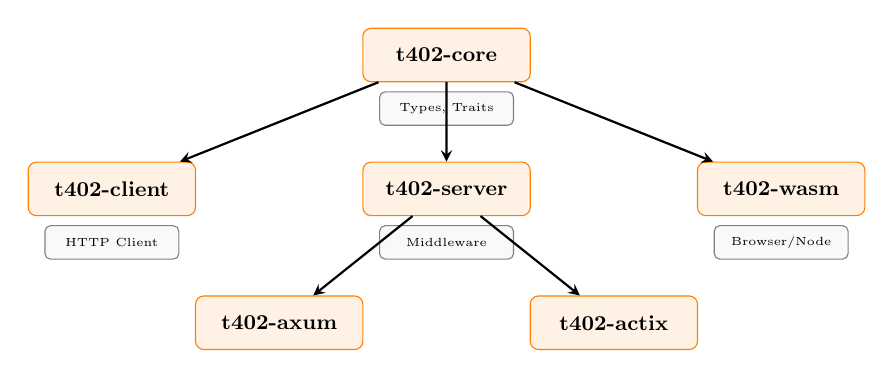
\begin{tikzpicture}[
    scale=0.85,
    transform shape,
    crate/.style={
        rectangle,
        rounded corners=3pt,
        minimum width=2.5cm,
        minimum height=0.8cm,
        draw=orange,
        fill=orange!10,
        font=\small\bfseries,
        align=center
    },
    feature/.style={
        rectangle,
        rounded corners=2pt,
        minimum width=2cm,
        minimum height=0.5cm,
        draw=gray,
        fill=gray!5,
        font=\tiny,
        align=center
    },
    arrow/.style={
        ->,
        thick,
        >=stealth
    }
]

% Core crate
\node[crate] (core) at (5,3) {t402-core};
\node[feature] at (5,2.2) {Types, Traits};

% Platform crates
\node[crate] (client) at (0,1) {t402-client};
\node[feature] at (0,0.2) {HTTP Client};

\node[crate] (server) at (5,1) {t402-server};
\node[feature] at (5,0.2) {Middleware};

\node[crate] (wasm) at (10,1) {t402-wasm};
\node[feature] at (10,0.2) {Browser/Node};

% Integration crates
\node[crate] (axum) at (2.5,-1) {t402-axum};
\node[crate] (actix) at (7.5,-1) {t402-actix};

% Arrows
\draw[arrow] (core) -- (client);
\draw[arrow] (core) -- (server);
\draw[arrow] (core) -- (wasm);
\draw[arrow] (server) -- (axum);
\draw[arrow] (server) -- (actix);

\end{tikzpicture}
\caption{Rust SDK Architecture}
\label{fig:rust-sdk}
\end{figure}

\subsubsection{Key Features}

\begin{lstlisting}[language=golang, caption={Rust SDK Usage Example (Rust syntax)}]
// Server middleware (Axum)
use t402_axum::T402Layer;

let app = Router::new()
    .route("/api/data", get(handler))
    .layer(T402Layer::new(config));

// Client
use t402_client::T402Client;

let client = T402Client::new(wallet);
let response = client
    .get("https://api.example.com/weather")
    .with_payment(usdt("0.01"))
    .send()
    .await?;
\end{lstlisting}

\subsubsection{WebAssembly Support}

The Rust SDK compiles to WebAssembly for:
\begin{itemize}
    \item Browser-based T402 clients
    \item Edge computing (Cloudflare Workers, Deno Deploy)
    \item Node.js native addon performance
\end{itemize}

%------------------------------------------------------------------------------
\subsection{Swift SDK}
\label{subsec:swift-sdk}

Native iOS and macOS support with modern Swift features:

\begin{lstlisting}[language=typescript, caption={Swift SDK Example (Swift syntax)}]
// Swift client usage
import T402

let client = T402Client(wallet: wallet)

let weather = try await client
    .request("https://api.example.com/weather")
    .pay(.usdt(0.01, network: .ethereum))
    .decode(WeatherResponse.self)

// SwiftUI integration
struct PaidContentView: View {
    @StateObject var payment = T402Payment()

    var body: some View {
        PaidContent(payment: payment) {
            ArticleView(article: article)
        } paywall: {
            PaywallView(amount: 0.10, asset: .usdt)
        }
    }
}
\end{lstlisting}

\subsubsection{Platform Integration}

\begin{itemize}
    \item \textbf{WalletConnect}: Native mobile wallet integration
    \item \textbf{Apple Pay Bridge}: Fiat-to-crypto via Apple Pay
    \item \textbf{Keychain}: Secure key storage
    \item \textbf{App Clips}: Lightweight payment flows
\end{itemize}

%------------------------------------------------------------------------------
\subsection{Kotlin SDK}
\label{subsec:kotlin-sdk}

Android-native SDK with Kotlin coroutines:

\begin{lstlisting}[language=typescript, caption={Kotlin SDK Example}]
// Kotlin Android usage
val client = T402Client.create(wallet)

val response = client.get("https://api.example.com/data")
    .pay(USDT.amount("0.01").on(Network.POLYGON))
    .await()

// Jetpack Compose integration
@Composable
fun PaidScreen(url: String) {
    val payment = rememberT402Payment()

    T402Gate(
        payment = payment,
        amount = 0.10.usdt(),
        content = { PremiumContent() },
        paywall = { PaywallDialog(onPay = payment::initiate) }
    )
}
\end{lstlisting}

%------------------------------------------------------------------------------
\subsection{C++ SDK}
\label{subsec:cpp-sdk}

Embedded systems and IoT devices require a lightweight C++ implementation:

\begin{itemize}
    \item \textbf{Minimal dependencies}: Only libcurl and OpenSSL
    \item \textbf{No heap allocation}: Static memory for constrained devices
    \item \textbf{FreeRTOS support}: IoT device integration
    \item \textbf{Arduino library}: Maker-friendly API
\end{itemize}

%==============================================================================
\section{Infrastructure Scaling}
\label{sec:infrastructure-future}
%==============================================================================

\subsection{Multi-Region Architecture}

\begin{figure}[htbp]
\centering
\begin{tikzpicture}[
    scale=0.75,
    transform shape,
    region/.style={
        rectangle,
        rounded corners=5pt,
        minimum width=3.5cm,
        minimum height=2.5cm,
        draw=#1,
        fill=#1!5,
        font=\small\bfseries,
        align=center
    },
    service/.style={
        rectangle,
        rounded corners=2pt,
        minimum width=1.2cm,
        minimum height=0.5cm,
        draw=gray,
        fill=white,
        font=\tiny,
        align=center
    },
    db/.style={
        cylinder,
        shape border rotate=90,
        aspect=0.3,
        minimum width=0.8cm,
        minimum height=0.6cm,
        draw=orange,
        fill=orange!10,
        font=\tiny,
        align=center
    },
    arrow/.style={
        <->,
        thick,
        gray
    }
]

% Regions
\node[region=t402blue] (us) at (0,0) {};
\node[above, font=\small\bfseries] at (0,1) {US-East};
\node[service] at (-0.8,0.3) {API};
\node[service] at (0.8,0.3) {API};
\node[db] at (0,-0.5) {DB};

\node[region=t402green] (eu) at (6,0) {};
\node[above, font=\small\bfseries] at (6,1) {EU-West};
\node[service] at (5.2,0.3) {API};
\node[service] at (6.8,0.3) {API};
\node[db] at (6,-0.5) {DB};

\node[region=t402purple] (apac) at (12,0) {};
\node[above, font=\small\bfseries] at (12,1) {APAC};
\node[service] at (11.2,0.3) {API};
\node[service] at (12.8,0.3) {API};
\node[db] at (12,-0.5) {DB};

% Global components
\node[rectangle, rounded corners=3pt, draw=orange, fill=orange!10, minimum width=10cm, minimum height=0.8cm, font=\small\bfseries] (cdn) at (6,3) {Global CDN \& Load Balancer};

\node[rectangle, rounded corners=3pt, draw=red, fill=red!10, minimum width=4cm, minimum height=0.8cm, font=\small\bfseries] (hsm) at (6,-3) {HSM Cluster};

% Connections
\draw[arrow] (us) -- (eu);
\draw[arrow] (eu) -- (apac);
\draw[arrow] (cdn) -- (us);
\draw[arrow] (cdn) -- (eu);
\draw[arrow] (cdn) -- (apac);
\draw[arrow, dashed] (us) -- (hsm);
\draw[arrow, dashed] (eu) -- (hsm);
\draw[arrow, dashed] (apac) -- (hsm);

\end{tikzpicture}
\caption{Multi-Region Facilitator Architecture}
\label{fig:multi-region}
\end{figure}

\subsubsection{Regional Deployment Goals}

\begin{table}[htbp]
\centering
\caption{Regional Deployment Targets}
\label{tab:regional-targets}
\begin{tabular}{@{}llcc@{}}
\toprule
\textbf{Region} & \textbf{Location} & \textbf{Latency Target} & \textbf{Status} \\
\midrule
US-East & Virginia & $<$50ms & Active \\
US-West & Oregon & $<$50ms & Planned \\
EU-West & Frankfurt & $<$50ms & Planned \\
APAC-East & Tokyo & $<$100ms & Planned \\
APAC-South & Singapore & $<$100ms & Planned \\
\bottomrule
\end{tabular}
\end{table}

%------------------------------------------------------------------------------
\subsection{Horizontal Scaling}

\begin{itemize}
    \item \textbf{Stateless API}: All state in distributed cache (Redis Cluster)
    \item \textbf{Auto-scaling}: Kubernetes HPA based on request rate
    \item \textbf{Connection pooling}: Shared RPC connections to blockchain nodes
    \item \textbf{Read replicas}: Database read scaling for verification queries
\end{itemize}

\subsubsection{Capacity Planning}

\begin{table}[htbp]
\centering
\caption{Scaling Milestones}
\label{tab:scaling-milestones}
\begin{tabular}{@{}rrrr@{}}
\toprule
\textbf{Tx/Day} & \textbf{API Pods} & \textbf{DB Size} & \textbf{Cache RAM} \\
\midrule
10,000 & 3 & 10 GB & 2 GB \\
100,000 & 10 & 100 GB & 8 GB \\
1,000,000 & 50 & 1 TB & 32 GB \\
10,000,000 & 200 & 10 TB & 128 GB \\
\bottomrule
\end{tabular}
\end{table}

%------------------------------------------------------------------------------
\subsection{Security Enhancements}

\subsubsection{Hardware Security Modules (HSM)}

Production hot wallets will migrate to HSM-backed key management:

\begin{itemize}
    \item \textbf{AWS CloudHSM}: FIPS 140-2 Level 3 compliance
    \item \textbf{Key rotation}: Automated monthly rotation
    \item \textbf{Multi-signature}: 2-of-3 threshold for high-value settlements
    \item \textbf{Audit logging}: All key operations logged to immutable store
\end{itemize}

\subsubsection{Rate Limiting Evolution}

\begin{lstlisting}[language=yaml, caption={Advanced Rate Limiting Configuration}]
rateLimiting:
  tiers:
    anonymous:
      rps: 10
      burst: 20
      dailyLimit: 1000
    authenticated:
      rps: 100
      burst: 200
      dailyLimit: 50000
    enterprise:
      rps: 1000
      burst: 5000
      dailyLimit: unlimited

  adaptive:
    enabled: true
    cpuThreshold: 80%
    memoryThreshold: 85%
    reductionFactor: 0.5

  ddosProtection:
    enabled: true
    provider: cloudflare
    challengeThreshold: 1000
\end{lstlisting}

%==============================================================================
\section{Standardization}
\label{sec:standardization}
%==============================================================================

\subsection{IETF Standardization}

The \tprotocol{} specification will be proposed as an Internet-Draft:

\subsubsection{Proposed RFC Structure}

\begin{enumerate}
    \item \textbf{RFC 9XXX: HTTP Payment Required (402) Protocol}
    \begin{itemize}
        \item Updates RFC 7231 with 402 semantics
        \item Defines \header{X-Payment} and \header{X-Payment-Response} headers
        \item Specifies scheme registry mechanism
    \end{itemize}

    \item \textbf{RFC 9XXY: Cryptocurrency Payment Schemes for HTTP 402}
    \begin{itemize}
        \item Defines \code{exact}, \code{up-to}, \code{permit2} schemes
        \item Network identifier format (CAIP-2)
        \item Authorization encoding standards
    \end{itemize}
\end{enumerate}

\subsubsection{Timeline}

\begin{enumerate}
    \item \textbf{Q3 2025}: Draft submission to IETF HTTP Working Group
    \item \textbf{Q4 2025}: Working group adoption
    \item \textbf{Q2 2026}: Last Call
    \item \textbf{Q4 2026}: RFC publication
\end{enumerate}

%------------------------------------------------------------------------------
\subsection{W3C Web Payments Integration}

Integration with W3C Payment Request API:

\begin{lstlisting}[language=typescript, caption={W3C Payment Request Integration}]
// Browser payment flow
const paymentRequest = new PaymentRequest(
  [
    {
      supportedMethods: 'https://t402.io/payment',
      data: {
        supportedNetworks: ['eip155:1', 'eip155:137'],
        supportedAssets: ['usdt', 'usdc'],
      }
    }
  ],
  {
    total: {
      label: 'API Access',
      amount: { currency: 'USDT', value: '0.10' }
    }
  }
);

const response = await paymentRequest.show();
const paymentHeader = response.details.paymentHeader;
// Use paymentHeader in X-Payment header
\end{lstlisting}

%------------------------------------------------------------------------------
\subsection{CAIP Alignment}

Full alignment with Chain Agnostic Improvement Proposals:

\begin{table}[htbp]
\centering
\caption{CAIP Alignment Status}
\label{tab:caip-alignment}
\begin{tabular}{@{}llc@{}}
\toprule
\textbf{CAIP} & \textbf{Description} & \textbf{Status} \\
\midrule
CAIP-2 & Blockchain ID Specification & Implemented \\
CAIP-10 & Account ID Specification & Implemented \\
CAIP-19 & Asset Type and ID & Planned \\
CAIP-122 & Sign-In-With-X & Planned \\
CAIP-25 & JSON-RPC Provider Request & Planned \\
\bottomrule
\end{tabular}
\end{table}

%==============================================================================
\section{Research Directions}
\label{sec:research-directions}
%==============================================================================

\subsection{Privacy-Preserving Payments}

\subsubsection{Zero-Knowledge Proofs}

Future protocol versions may incorporate ZK proofs for:

\begin{itemize}
    \item \textbf{Payment amount privacy}: Prove payment $\geq$ threshold without revealing exact amount
    \item \textbf{Identity privacy}: Prove wallet membership in allowed set (ZK set membership)
    \item \textbf{Compliance proofs}: Prove KYC completion without revealing identity
\end{itemize}

\begin{figure}[htbp]
\centering
\begin{tikzpicture}[
    scale=0.85,
    transform shape,
    box/.style={
        rectangle,
        rounded corners=3pt,
        minimum width=2.5cm,
        minimum height=1cm,
        draw=#1,
        fill=#1!10,
        font=\small\bfseries,
        align=center
    },
    arrow/.style={
        ->,
        thick,
        >=stealth
    }
]

\node[box=t402blue] (prover) at (0,0) {Client\\(Prover)};
\node[box=t402green] (verifier) at (6,0) {Provider\\(Verifier)};
\node[box=t402purple] (proof) at (3,2) {ZK Proof:\\$payment \geq \$0.10$};

\draw[arrow] (prover) -- node[left, font=\tiny] {Generate} (proof);
\draw[arrow] (proof) -- node[right, font=\tiny] {Verify} (verifier);
\draw[arrow, dashed] (verifier) -- node[below, font=\tiny] {Access granted} (prover);

\node[below=0.5cm of prover, font=\tiny, align=center] {Knows: exact amount\\Reveals: nothing};
\node[below=0.5cm of verifier, font=\tiny, align=center] {Learns: amount $\geq$ 0.10\\Not: exact amount};

\end{tikzpicture}
\caption{Zero-Knowledge Payment Verification}
\label{fig:zk-payments}
\end{figure}

%------------------------------------------------------------------------------
\subsection{Cross-Chain Atomic Payments}

Research into atomic cross-chain payments for multi-chain scenarios:

\begin{itemize}
    \item \textbf{Hash Time-Locked Contracts (HTLC)}: Trustless cross-chain swaps
    \item \textbf{Layered settlements}: L2-to-L2 transfers via bridges
    \item \textbf{Intent-based payments}: Express payment intent, let solvers optimize execution
\end{itemize}

%------------------------------------------------------------------------------
\subsection{AI Agent Integration Research}

\subsubsection{Autonomous Agent Economics}

As AI agents become economic actors, research focuses on:

\begin{enumerate}
    \item \textbf{Agent identity}: How do agents prove identity across services?
    \item \textbf{Budget management}: Safe delegation of spending authority
    \item \textbf{Reputation systems}: Trust scoring for agent-to-agent commerce
    \item \textbf{Dispute resolution}: Automated arbitration for agent disputes
\end{enumerate}

\subsubsection{Multi-Agent Payment Protocols}

\begin{lstlisting}[language=json, caption={Multi-Agent Payment Coordination}]
{
  "taskId": "research-task-123",
  "coordinator": "agent:researcher-001",
  "budget": {
    "total": "50.00",
    "asset": "usdt",
    "network": "eip155:137"
  },
  "subtasks": [
    {
      "agent": "agent:data-collector",
      "allocation": "20.00",
      "services": ["https://api.weather.com/*"]
    },
    {
      "agent": "agent:analyzer",
      "allocation": "25.00",
      "services": ["https://api.openai.com/*"]
    }
  ],
  "settlement": "atomic",
  "deadline": "2025-01-20T00:00:00Z"
}
\end{lstlisting}

%------------------------------------------------------------------------------
\subsection{Streaming Payments}

Research into continuous payment streams for real-time services:

\begin{itemize}
    \item \textbf{Superfluid integration}: Per-second payment streams
    \item \textbf{Dynamic rate adjustment}: Auto-adjust stream rate based on usage
    \item \textbf{Stream aggregation}: Combine multiple micro-streams for efficiency
\end{itemize}

%==============================================================================
\section{Community and Ecosystem}
\label{sec:community}
%==============================================================================

\subsection{Developer Ecosystem}

\begin{itemize}
    \item \textbf{SDK contributions}: Open-source community SDKs (Elixir, Scala, PHP)
    \item \textbf{Integration templates}: Ready-to-deploy templates for popular frameworks
    \item \textbf{Developer grants}: Funding for innovative T402 applications
    \item \textbf{Hackathons}: Quarterly hackathons with prizes
\end{itemize}

\subsection{Governance}

Long-term protocol governance considerations:

\begin{enumerate}
    \item \textbf{Technical Steering Committee}: Protocol evolution decisions
    \item \textbf{Specification process}: RFC-style proposal and review
    \item \textbf{Reference implementation}: Canonical SDK implementations
    \item \textbf{Certification program}: Verified compliant implementations
\end{enumerate}

\subsection{Interoperability Initiatives}

\begin{itemize}
    \item \textbf{Payment gateway bridges}: Connect T402 to traditional payment rails
    \item \textbf{Cross-protocol payments}: Interoperability with Lightning, Bolt12
    \item \textbf{Identity federation}: Accept multiple identity standards (SIWx, Verifiable Credentials)
\end{itemize}

%==============================================================================
\section{Conclusion}
\label{sec:future-conclusion}
%==============================================================================

The \tprotocol{} protocol has established a foundation for HTTP-native cryptocurrency payments. The roadmap outlined in this chapter charts a path toward:

\begin{itemize}
    \item \textbf{Enhanced flexibility}: Up-To metering, subscriptions, and refunds
    \item \textbf{Broader reach}: New SDKs for Rust, Swift, Kotlin, and C++
    \item \textbf{Global scale}: Multi-region infrastructure with enterprise-grade security
    \item \textbf{Industry adoption}: IETF and W3C standardization
    \item \textbf{Advanced capabilities}: Privacy, cross-chain, and AI agent integration
\end{itemize}

The protocol's modular architecture ensures these enhancements can be adopted incrementally, maintaining backward compatibility while enabling continuous innovation in the intersection of web services and blockchain payments.

\begin{infobox}[Contributing to T402]
The \tprotocol{} protocol is open source. Contributions are welcome:
\begin{itemize}
    \item \textbf{GitHub}: \url{https://github.com/t402-io/t402}
    \item \textbf{Documentation}: \url{https://docs.t402.io}
    \item \textbf{Discussions}: \url{https://github.com/t402-io/t402/discussions}
\end{itemize}
\end{infobox}
